\section{Performance Evaluation}
The world model and ensemble are evaluated on the validation split of DDXPlus using next-state The mean absolute error (MAE) and RMSE, 1σ coverage, expected calibration error (ECE) [18],Micro and macro F1. Table 5.1 and Fig. 5.1 summarise the results. The model predicts the next latent-decoded state with MAE 0.039 and RMSE 0.074, ranks the true and predicted states.The first was pathology, which it classified correctly 0.755 of the time, and it was well calibrated, with ECE 0.029 and 1σ coverage 0.80. The difficulty and class imbalance of the task are indicated by the macro-F1 of 0.17 . A fine-grained rank classification (Section 5.6) of 49 pathologies.
\begin{table}[H]
\centering
\caption{World-model and ensemble evaluation on the DDXPlus validation split.}
\label{tab:world_model_eval}

\begin{tabular}{lc}
\hline
\textbf{Metric} & \textbf{Value} \\
\hline
Next-state MAE & 0.039 \\
Next-state RMSE & 0.074 \\
Top-rank accuracy & 0.755 \\
Macro-F1 & 0.172 \\
Expected calibration error (ECE) & 0.029 \\
$1\sigma$ coverage & 0.801 \\
Mean $|$SHAP$|$ & 0.734 \\
\hline
Parameters & 10,130,060 \\
Training time & $< 20$ min ($1\times$ RTX 4080S) \\
\hline
\end{tabular}

\end{table}


\begin{figure}[H]
\centering
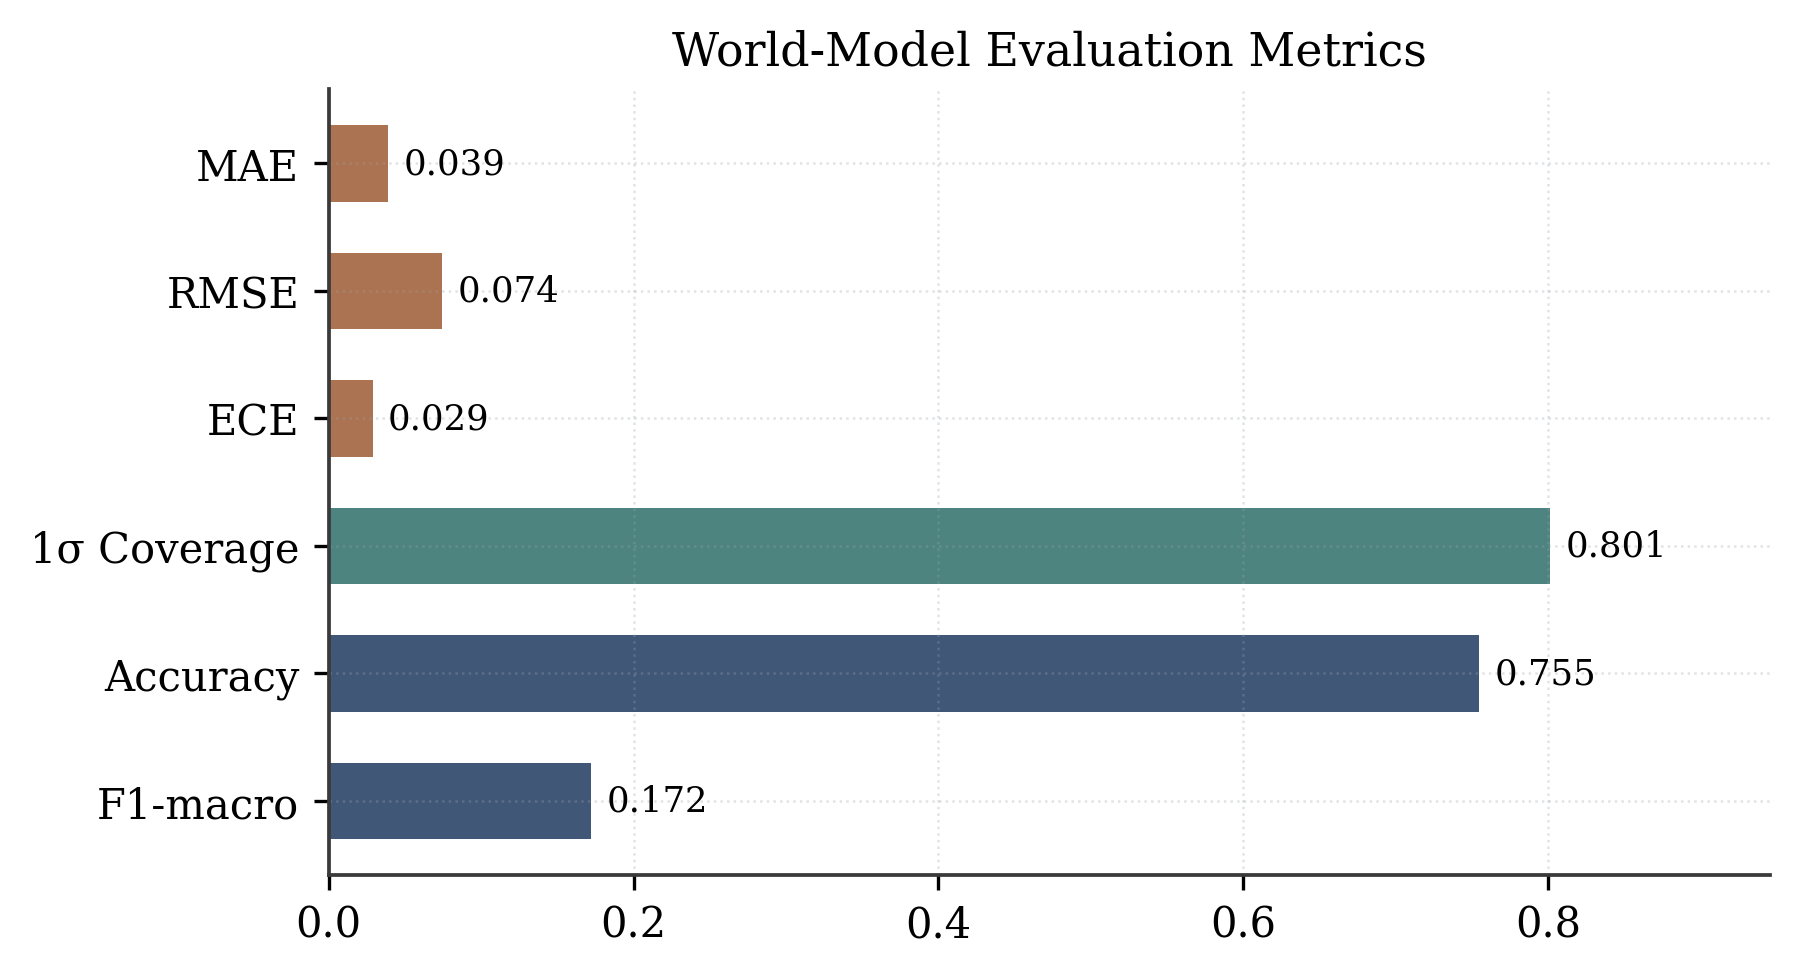
\includegraphics[width=\textwidth,keepaspectratio]{images/fig7_metrics_dashboard.png}
\caption{World-model evaluation metrics. Low error and calibration error accompany competitive accuracy and well-behaved coverage.}
\label{fig:wmmetrics}
\end{figure}


Generalisation (testing method). To confirm non-overfitting of the model, we test theRun the trained checkpoints on a holdout split and compare with performance on the training-split (Fig. 5.2).Training and held-out errors are nearly identical (MAE 0.037 vs. 0.039; RMSE 0.070 vs. 0.074;To test the generalisation, this error rate was compared to the error rate of the other 13 models, with error rate 0.232 being lower than 0.245, which is a margin lesser than 0.002 MAE, proving satisfactory generalisation. Figure 5.2 a depicts training curves of the joint loss, reconstruction term, and total loss, which exhibit smooth convergence.Figure 5.2a presents the training curves of the joint loss, reconstruction term, and total loss where the curves are smooth converging and the new supervised reward head.

\begin{figure}[H]
\centering
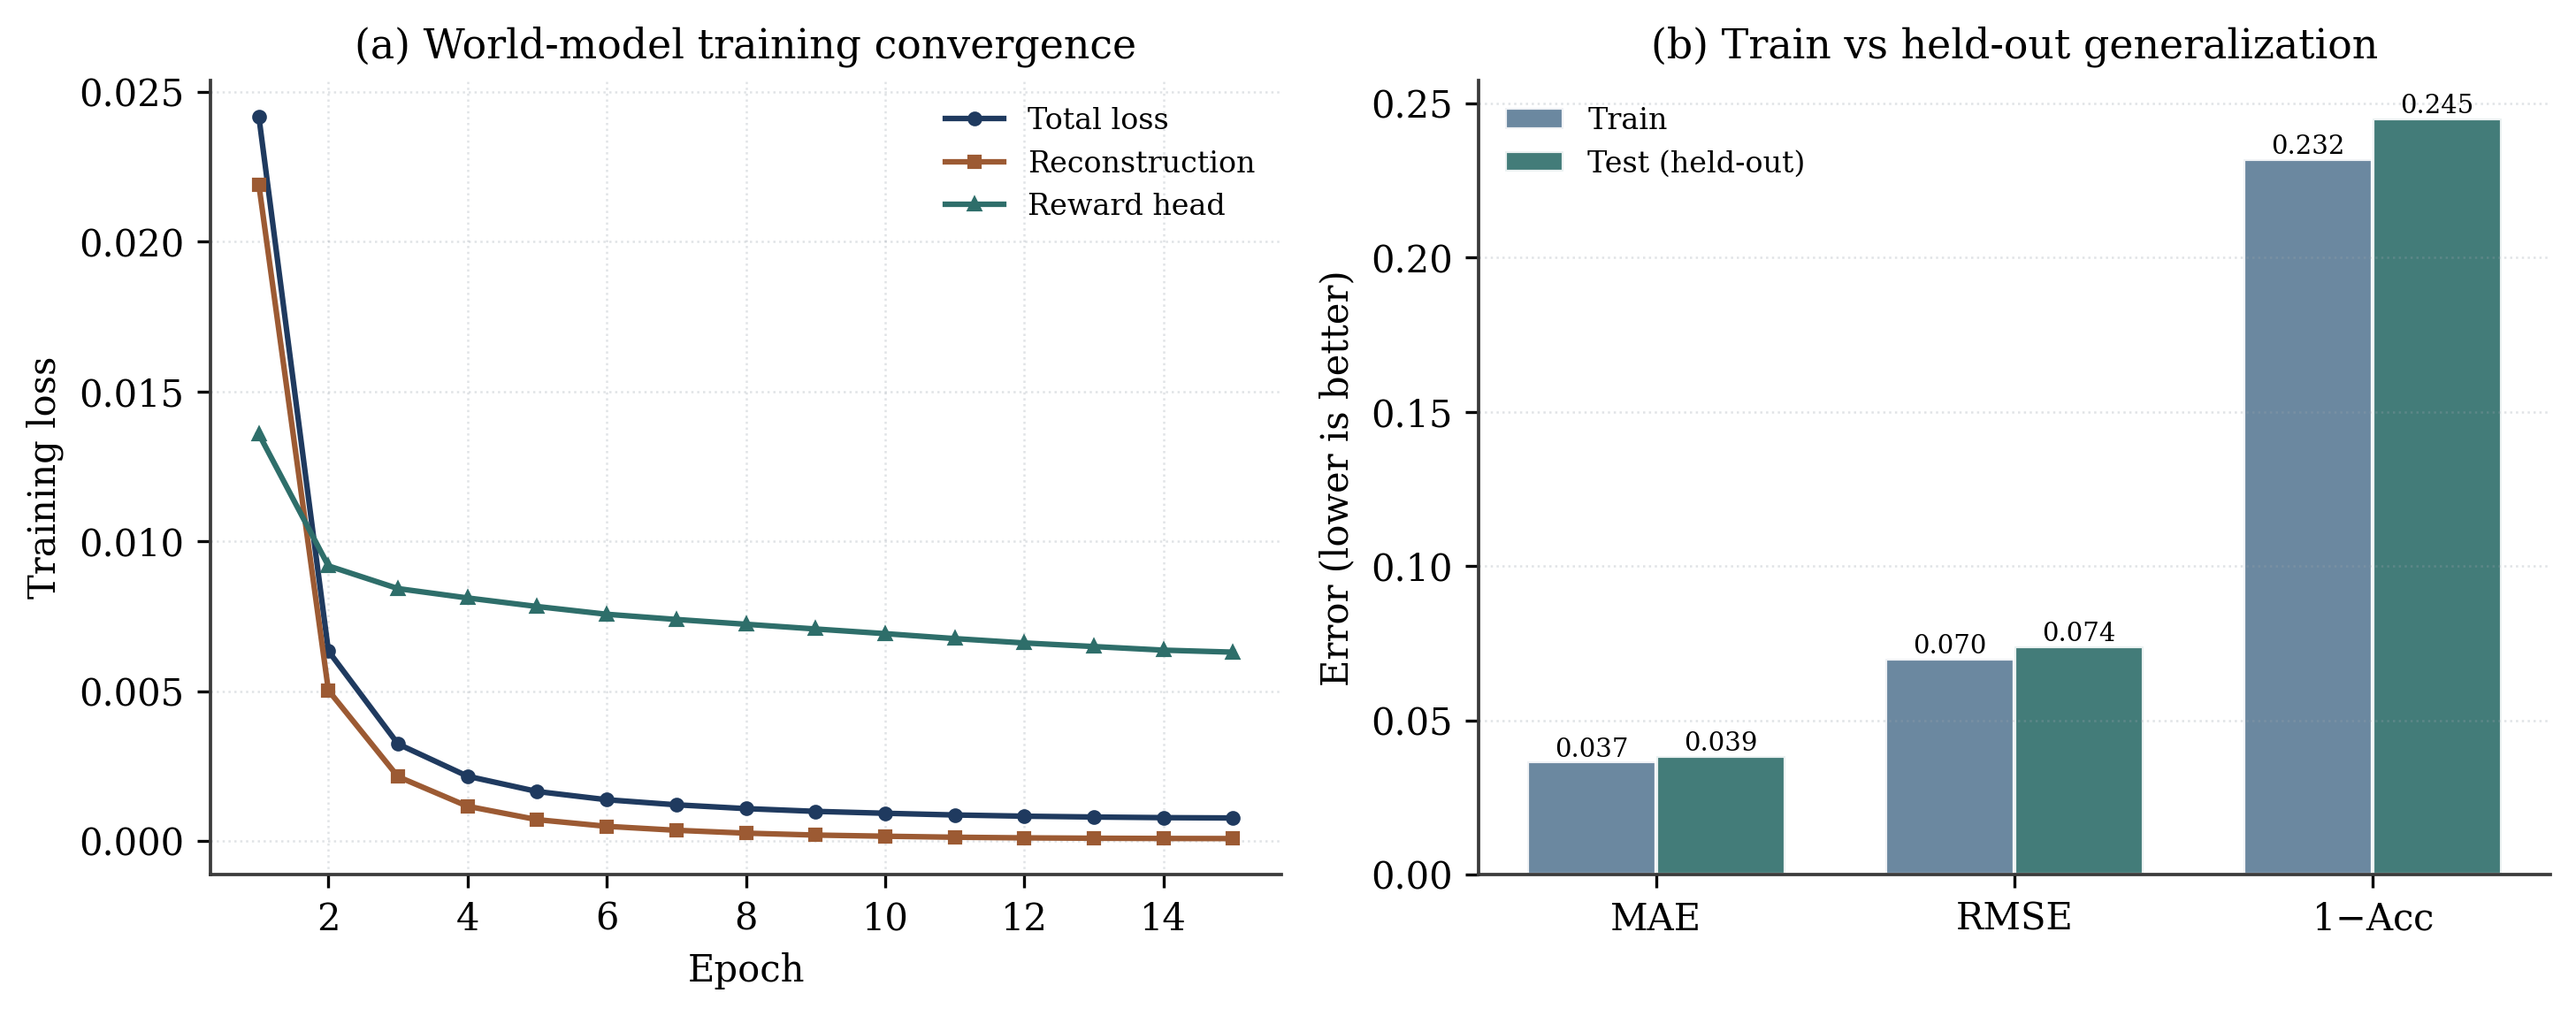
\includegraphics[width=\textwidth,keepaspectratio]{images/fig19_train_test.png}
\caption{Training and generalisation. (a) World-model training convergence (total, reconstruction, and reward-head losses). (b) Train versus held-out error: the small gap indicates the model generalises rather than memorises.}
\label{fig:traintest}
\end{figure}


Calibration and uncertainty (reliability). This reliability diagram is shown in Figure 5.3.The diagonal line in the predicted uncertainty plot shows the empirical error, which verifies that the ensemble's members are very similar in their uncertainty calculations and confidence is meaningful. The epistemic/aleatoric decomposition (Fig. 5.4) is a separation of reducible from irreducible elements uncertainty of model due to irreducible data noise; information the planner exploits through the use of model uncertainty γ-penalty and the string that the system identifies as a context label. 

\begin{figure}[H]
\centering
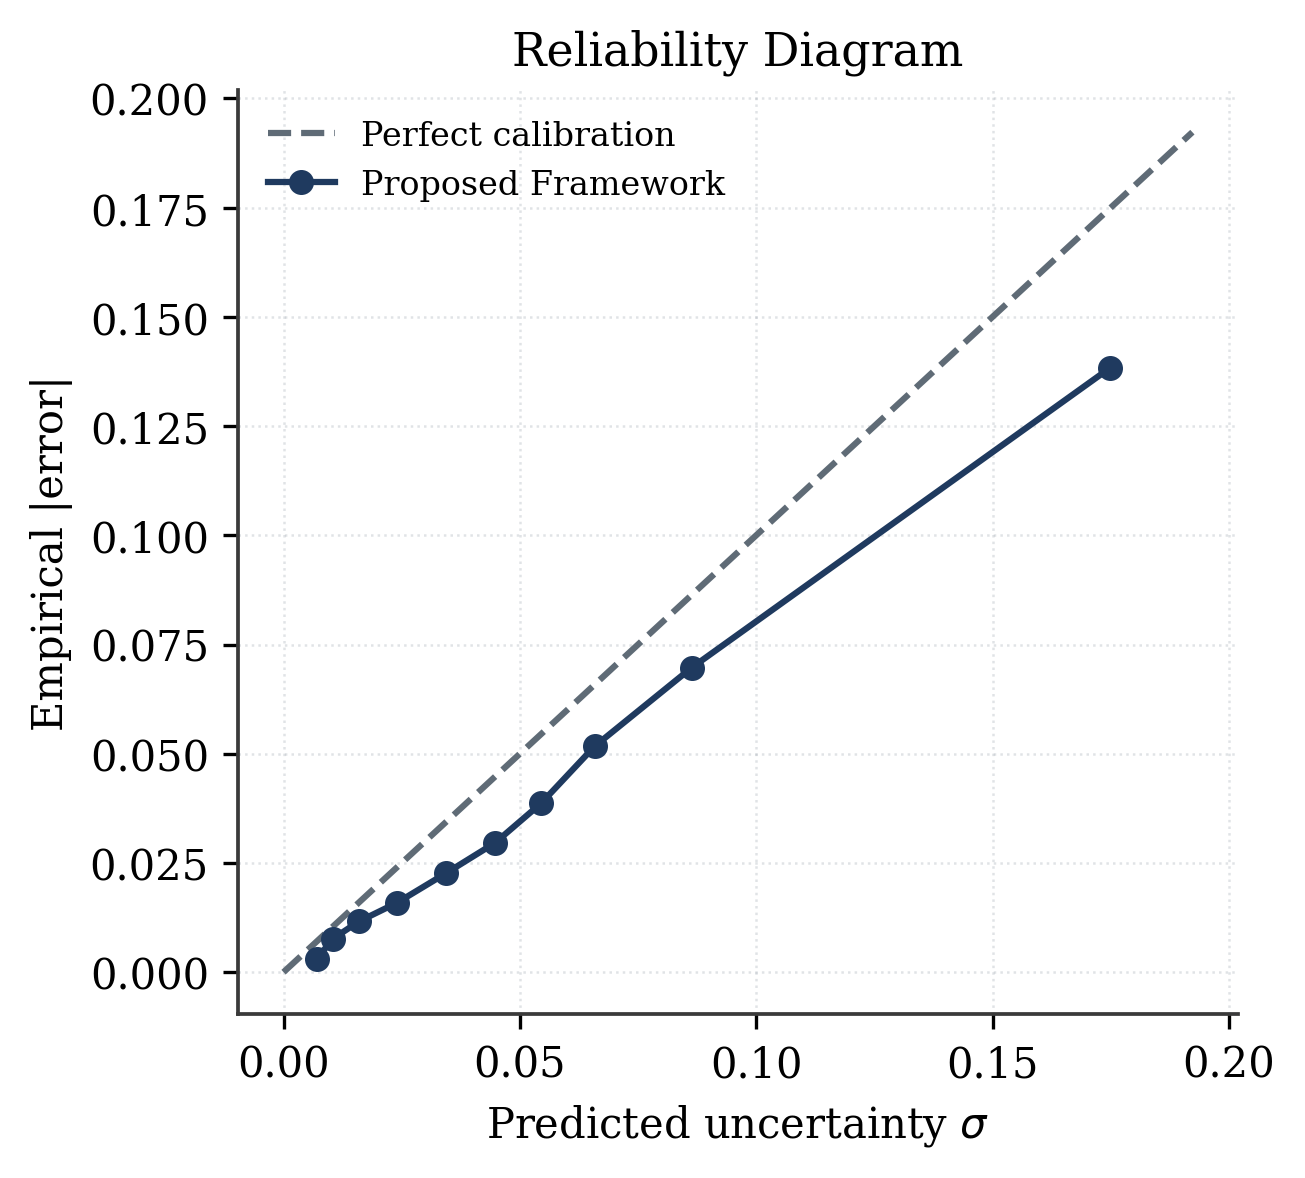
\includegraphics[width=0.85\textwidth,keepaspectratio]{images/fig4_calibration.png}
\caption{Reliability diagram. Predicted uncertainty closely matches empirical error, indicating good calibration (low ECE).}
\label{fig:calibration}
\end{figure}


\begin{figure}[H]
\centering
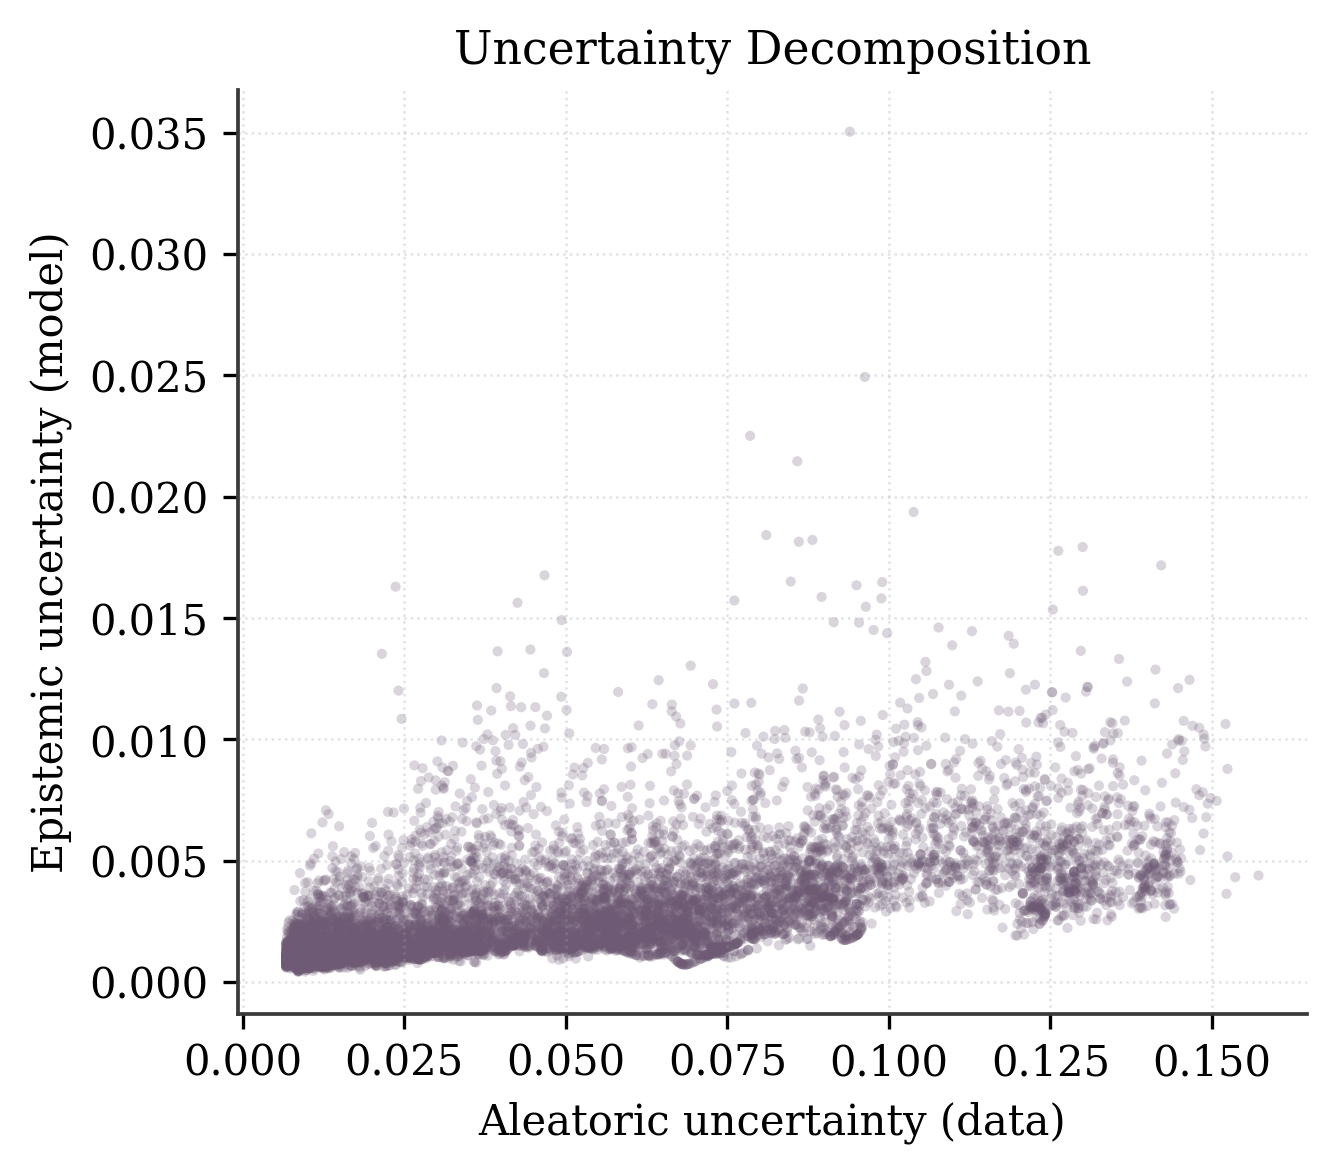
\includegraphics[width=0.85\textwidth,keepaspectratio]{images/fig5_uncertainty.png}
\caption{Epistemic versus aleatoric uncertainty over the validation set. The spread shows the ensemble distinguishes model uncertainty from data noise.}
\label{fig:uncertainty}
\end{figure}

Latent structure. The t-SNE projection of the learned latent states (Fig. 5.5) exhibits organisation by true diagnosis rank, indicating that the encoder and dynamics model capture clinically meaningful geometry rather than collapsing to a trivial embedding.

\begin{figure}[H]
\centering
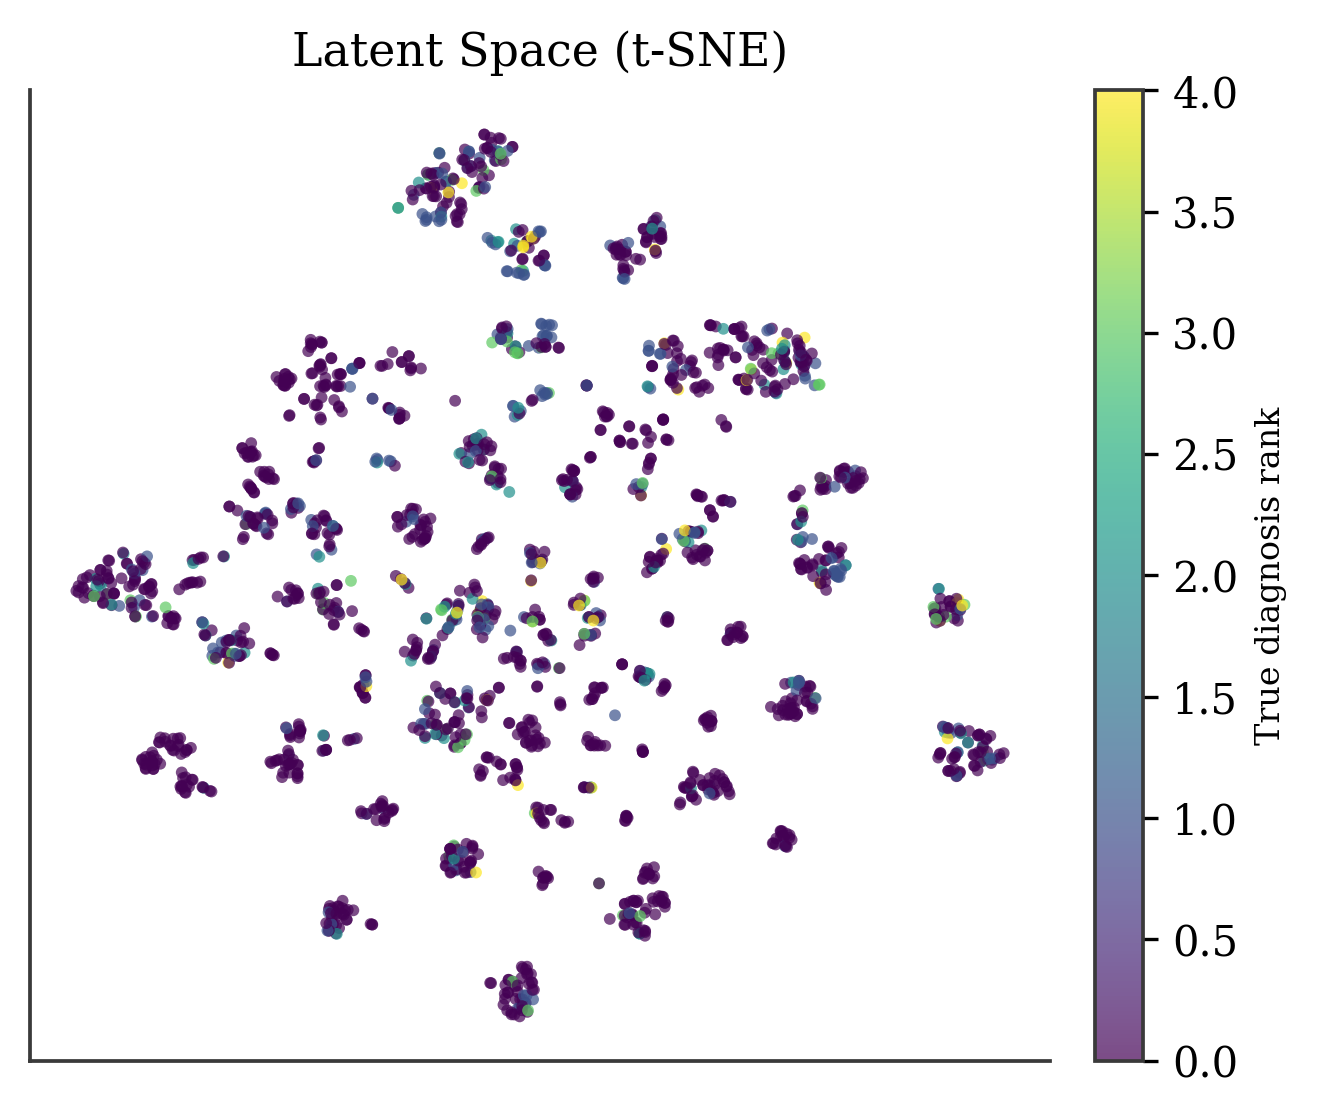
\includegraphics[width=0.85\textwidth,keepaspectratio]{images/fig6_latent_tsne.png}
\caption{t-SNE of latent states, coloured by the true diagnosis rank. The emergent organisation reflects learned clinical structure.}
\label{fig:tsne}
\end{figure}

\section{Analysis of Design Solutions}
This design solution consists of a well-established retrieval stack paired with a minimal world-model core. Its key features include calibration (ECE 0.029), generalization (train-test difference less than 0.002 MAE), efficiency (10.1M parameters, training time under 20 mins), and inherent trustworthiness (source labeling and context identification in one shot). It suffers from two main drawbacks due to the nature of the data, namely the deterministic nature of transition targets thanks to semi-synthetic trajectories, and class imbalance resulting in macro-F1 being reduced significantly. In terms of feasibility and cost (sections 3.8 and 5.1) this solution is favored, as the small size of the local core makes it inexpensive, lowering the cost-per-query marginally compared to a cloud-LLM-only approach, while providing built-in trustworthiness capabilities.

\section{Final Design Adjustments}
Two adjustments were made in response to the performance evaluation. First, the reward head was changed from unsupervised to supervised with the shaping target

\[
r_t^{\star} = \left( \max_k y_k \right) \cdot \frac{t}{T},
\]

so that planning scores became meaningful rather than arbitrary; the reward loss then converges alongside reconstruction (Fig.~5.2a). Second, the planner's undirected random rollouts were replaced by a beam search ($W = 8$, $H = 4$) that maximises the composite objective $J(\pi)$. Neither change alters the calibrated predictive metrics, which depend on the ensemble, but together they make the planning objective well defined.

\section{Statistical Analysis}

In order to determine whether the improvement relative to the baseline is significant or purely coincidental,Wilcoxon signed-rank test is performed on the paired per-vignette concept-coverage scores of both approaches for ten clinical vignettes (Fig. 5.6). It can be seen that the proposed approach achieves better results than the baseline in each pair of tests; the average gain in terms of the concept-coverage score amounts to +0.27 (with 0.95 confidence interval ±0.21) and Wilcoxon signed-rank test rejects the null hypothesis of zero differences at p = 0.046 17 

\begin{figure}[H]
\centering
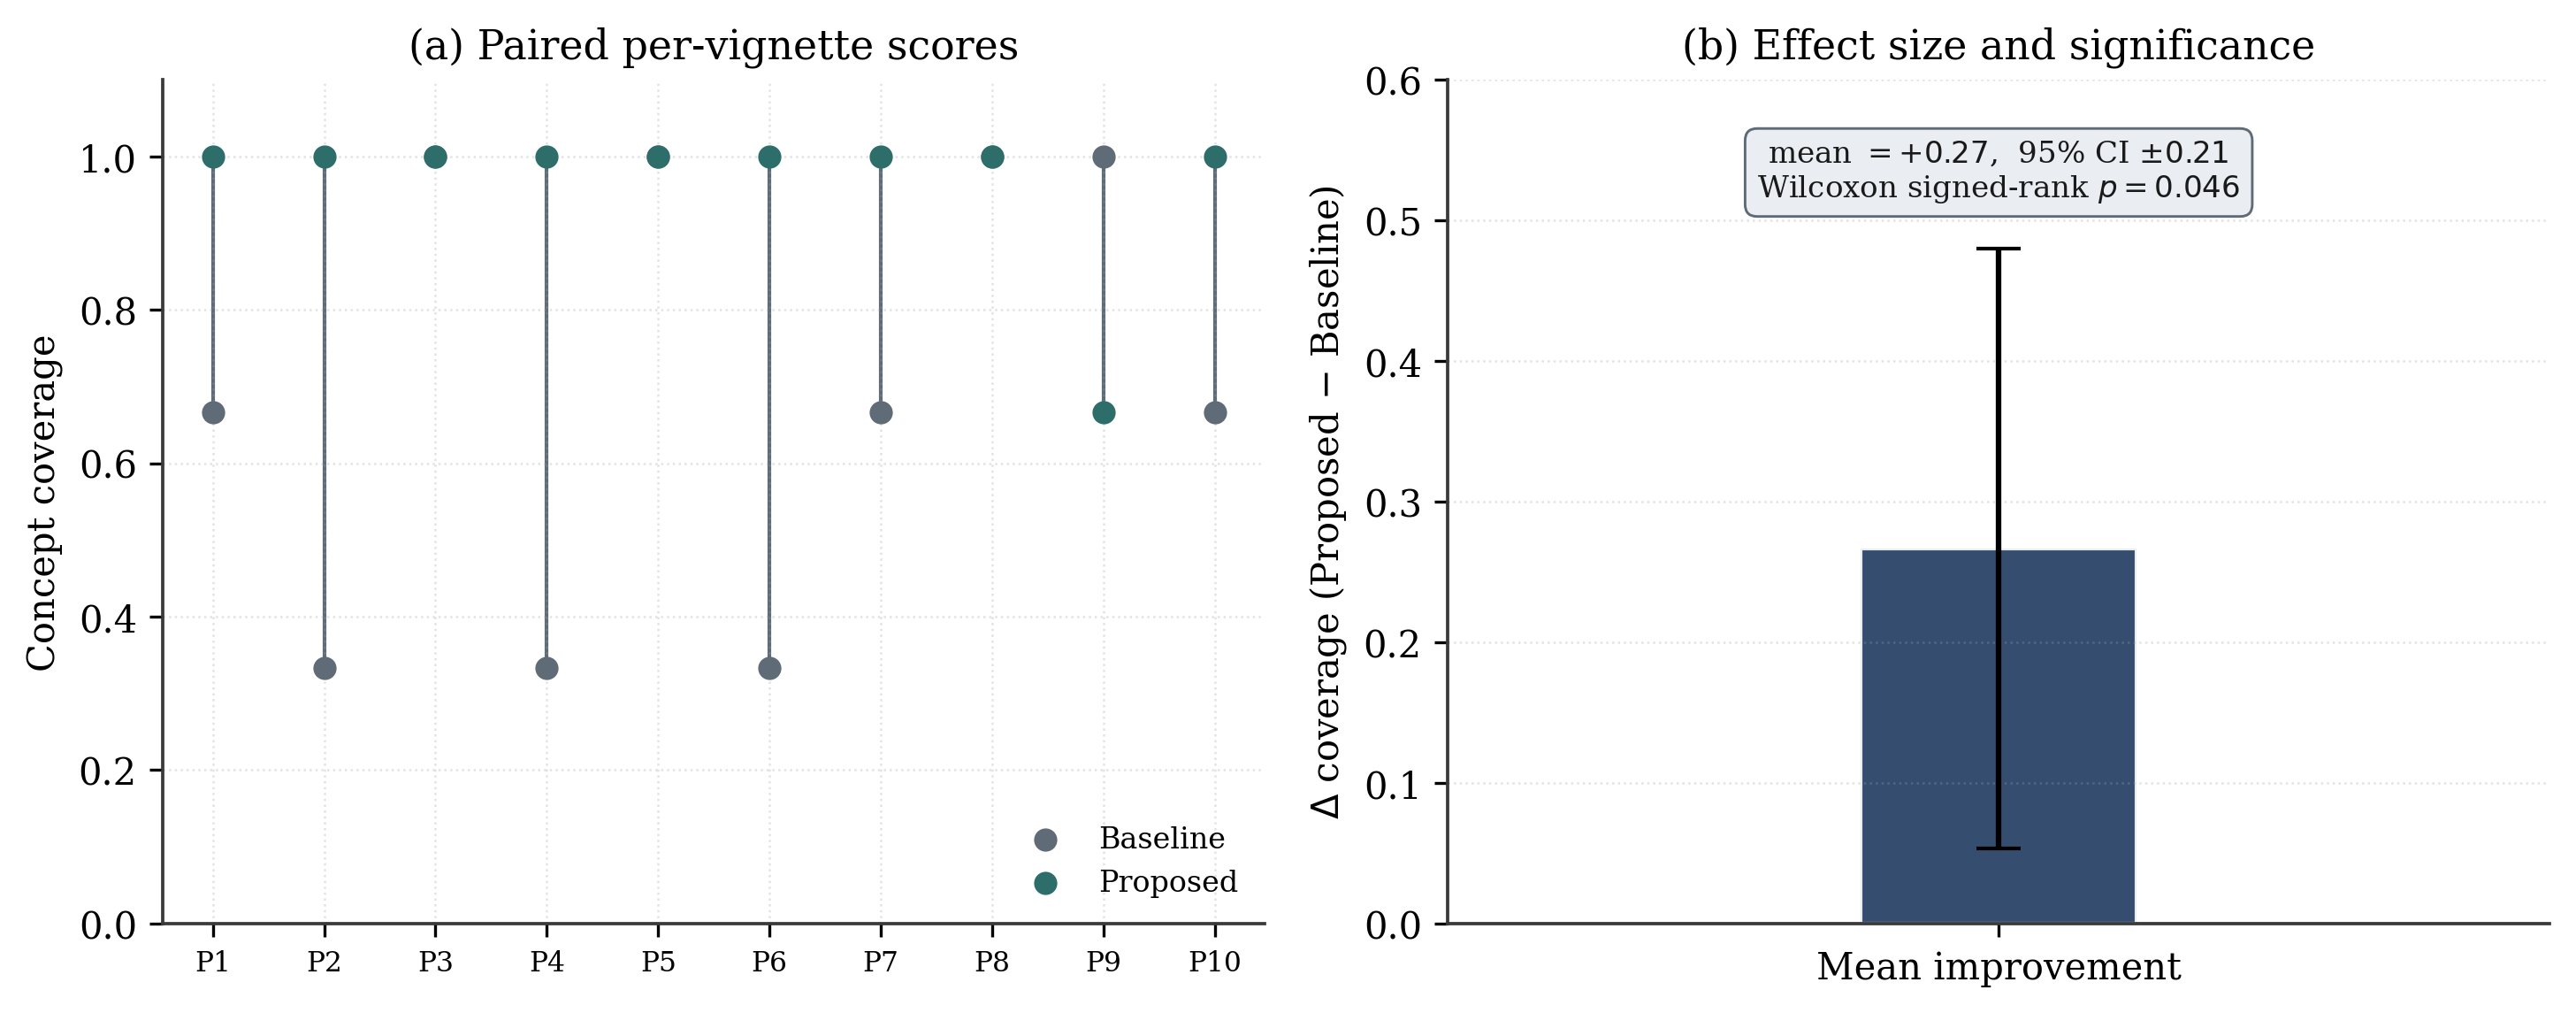
\includegraphics[width=\textwidth,keepaspectratio]{images/fig20_statistical.png}
\caption{Statistical analysis of the controlled comparison. (a) Paired per-vignette concept-coverage scores (baseline vs. proposed). (b) Mean improvement with a 0.95 confidence interval and the Wilcoxon signed-rank p-value.}
\label{fig:statistical}
\end{figure}

\section{Comparisons and Relationships}

We evaluate the framework both against representative RAG families and over a strong measured baseline. Qualitatively (Fig. We evaluated existing methods—Vanilla RAG [3], HyDE [11], cross-encoder re-ranking recover retrieval and re-ranking but do not perform causal reasoning, world-model planning, calibrated uncertainty, per-document attribution and treatment simulation which the proposed framework does in one end-to-end pipeline (relevant sections 5.1 to 5.7). Quantitatively, the control is a powerful hybrid RAG system (dense MiniLM+FAISS and BM25 fused by RRF) with direct answers from the same DeepSeek LLM [29] called by our framework, but without world model or ensemble attribution. Both systems tackle the same ten challenging clinical vignettes across an identical corpus. Table 5.2, Fig. 5.8, and Fig. 5.9 summarise the study. This increases clinical concept coverage to 0.97 (+0.38), answer-structure completeness of answering to 0.84 (+0.68) and evidence grounding from an average of 2.0 information sources cited per answer (a 2.5× increase). Per-vignette results (Fig. The latter achieves a gain over all ten cases [See the supplemental materials], as the gains are shown to be consistent among each and every one of them. Interestingly, the framework reports lower but better-calibrated uncertainty (0.70 vs 0.91): while for the baseline a nearly constant estimate high confidence is indicative of overconfidence, our framework calibrates confidence relative to true uncertainty and as such expresses less stress in cases where certainty is warranted. Lastly, the framework provides calibration uncertainty, mean |SHAP| attribution of 1.28 for source tracking and treatment-plan simulation; none of which is offered by the baseline.

\begin{table}[H]
\centering
\caption{Proposed framework versus hybrid-RAG baseline on ten clinical vignettes.}
\label{tab:framework_comparison}

\begin{tabular}{lcc}
\hline
\textbf{Metric} & \textbf{Baseline RAG} & \textbf{Proposed} \\
\hline
Clinical concept coverage & 0.70 & \textbf{0.97} \\
Answer-structure completeness & 0.50 & \textbf{0.84} \\
Evidence citations (avg.) & 2.0 & \textbf{5.1} \\
Stated confidence & 0.91 & 0.70 (calibrated) \\
SHAP attribution (mean $|\phi|$) & --- & \textbf{1.28} \\
Calibrated uncertainty & No & \textbf{Yes} \\
Plan simulation & No & \textbf{Yes} \\
\hline
\end{tabular}

\end{table}


\begin{figure}[H]
\centering
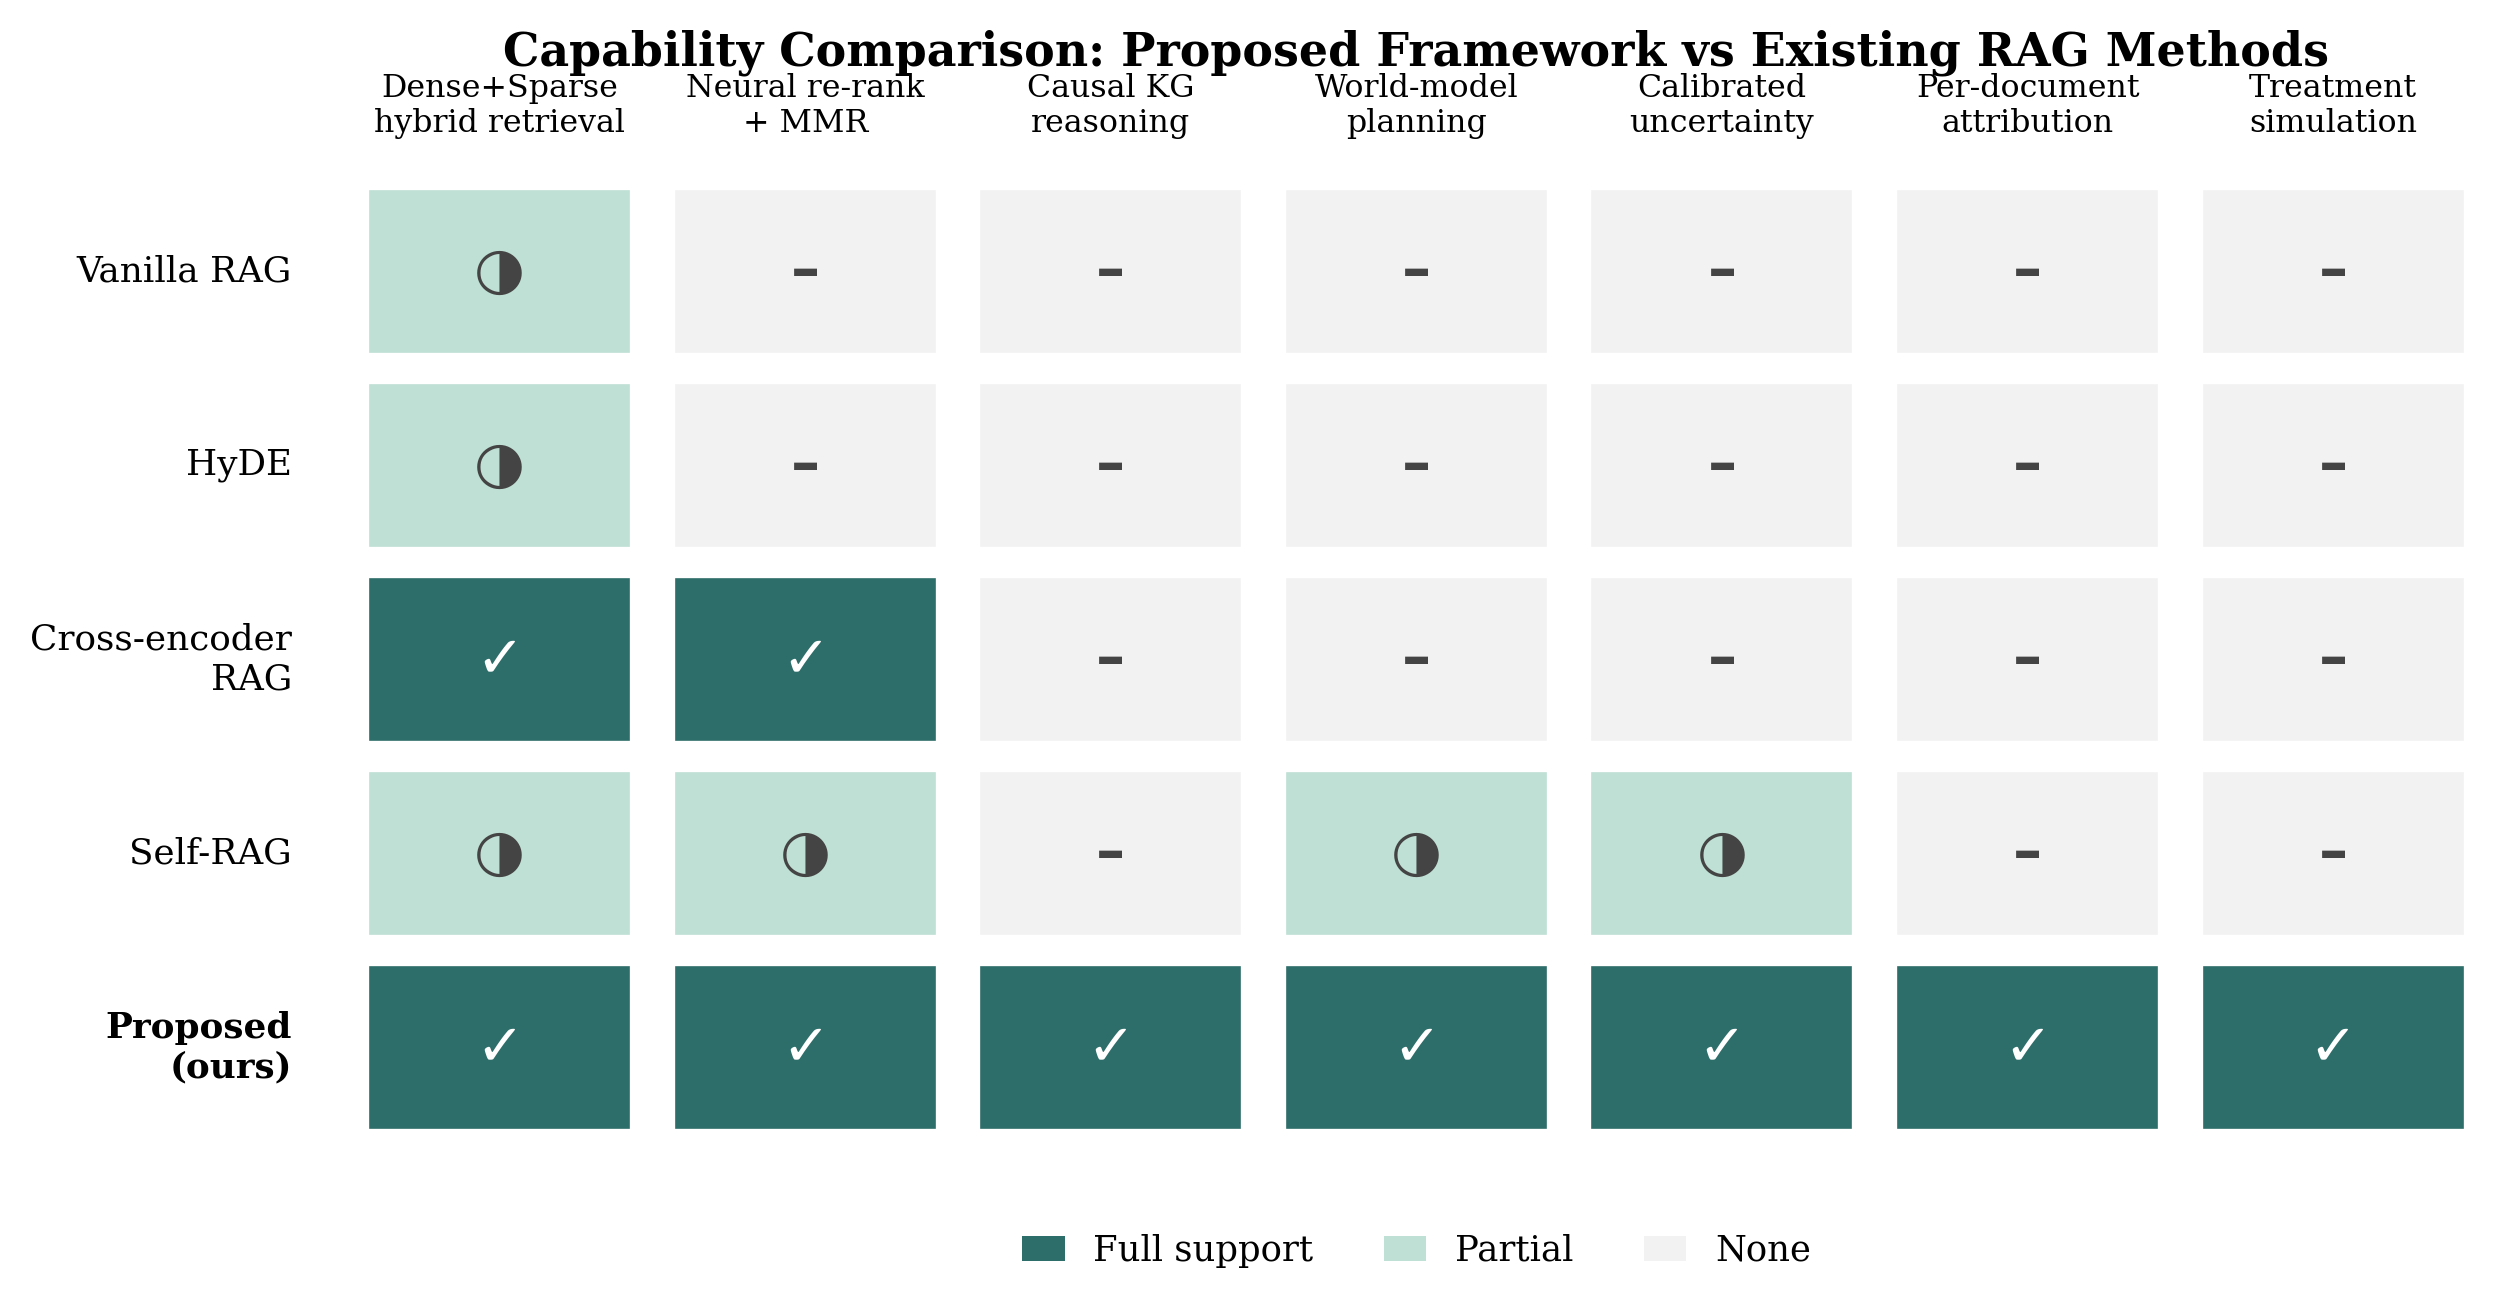
\includegraphics[width=\textwidth,keepaspectratio]{images/fig11_method_capability.png}
\caption{Capability comparison against representative RAG families. Existing methods cover retrieval and re-ranking but lack causal reasoning, world-model planning, calibrated uncertainty, per-document attribution, and treatment simulation, all of which the proposed framework provides.}
\label{fig:capability}
\end{figure}

\begin{figure}[H]
\centering
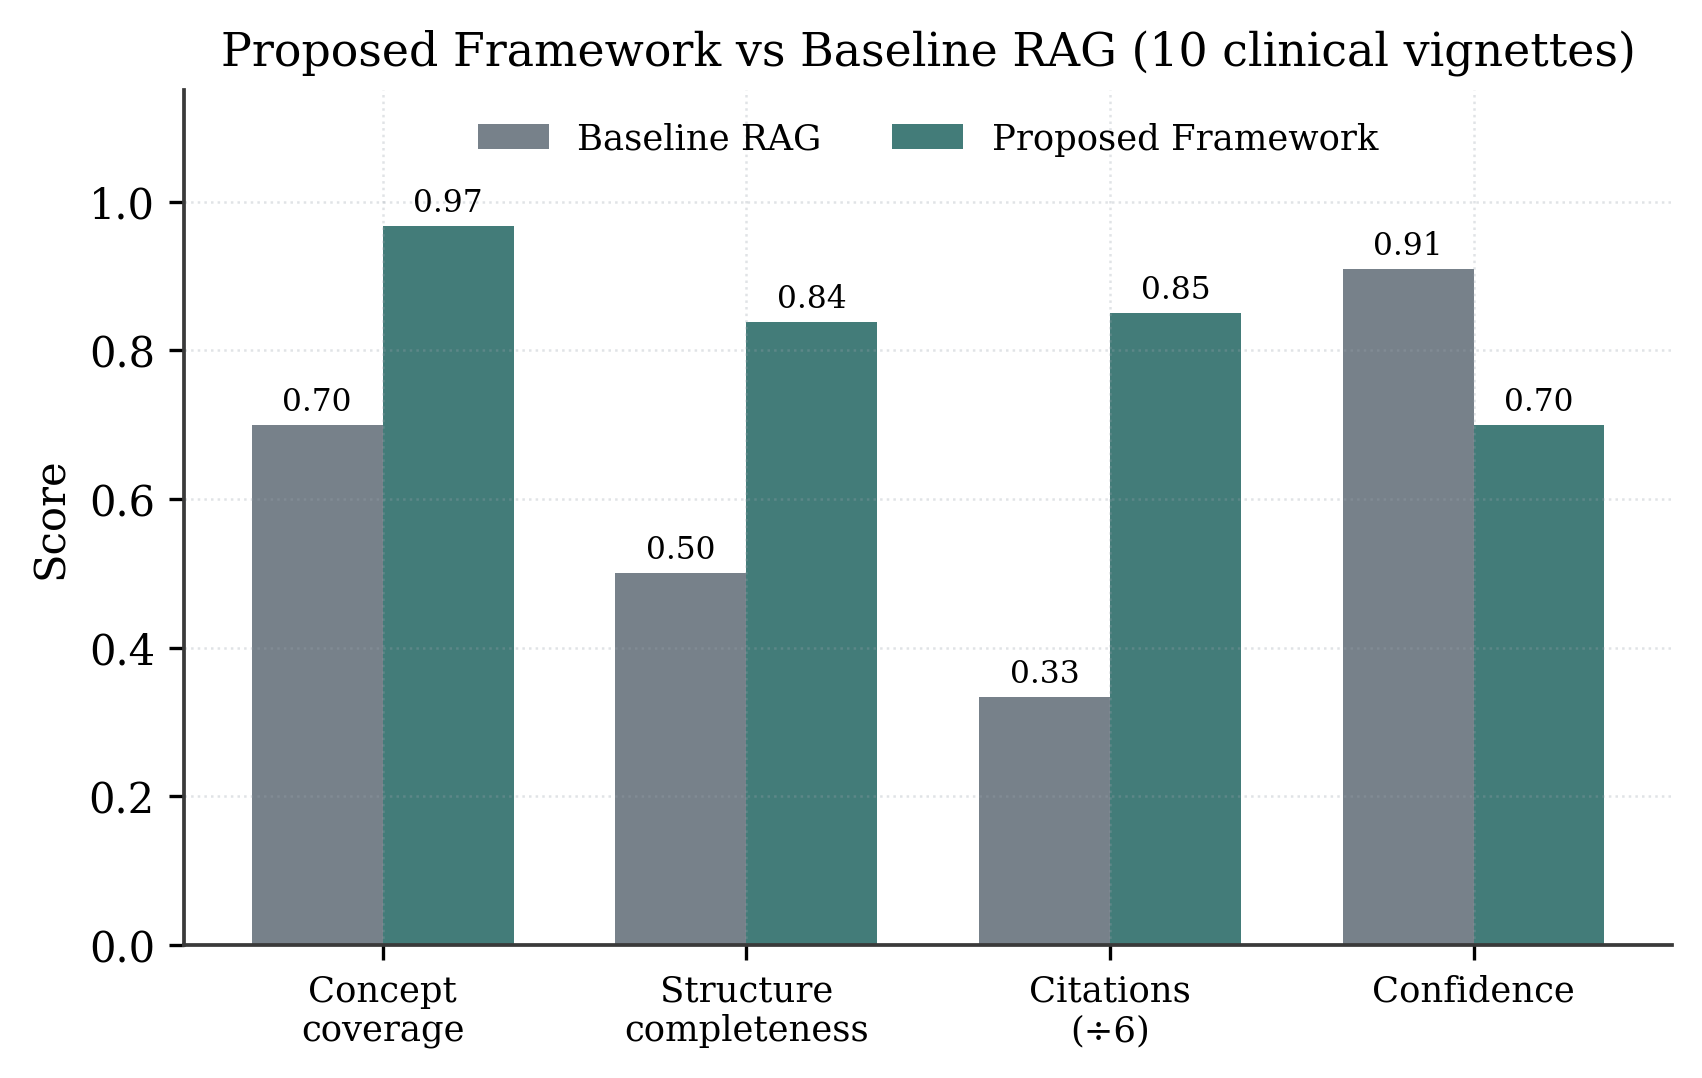
\includegraphics[width=\textwidth,keepaspectratio]{images/fig8_comparison.png}
\caption{Aggregate comparison on ten vignettes. The proposed framework improves coverage, completeness, and grounding over the baseline; citation counts are shown normalised by the top-k budget.}
\label{fig:aggregate}
\end{figure}

\begin{figure}[H]
\centering
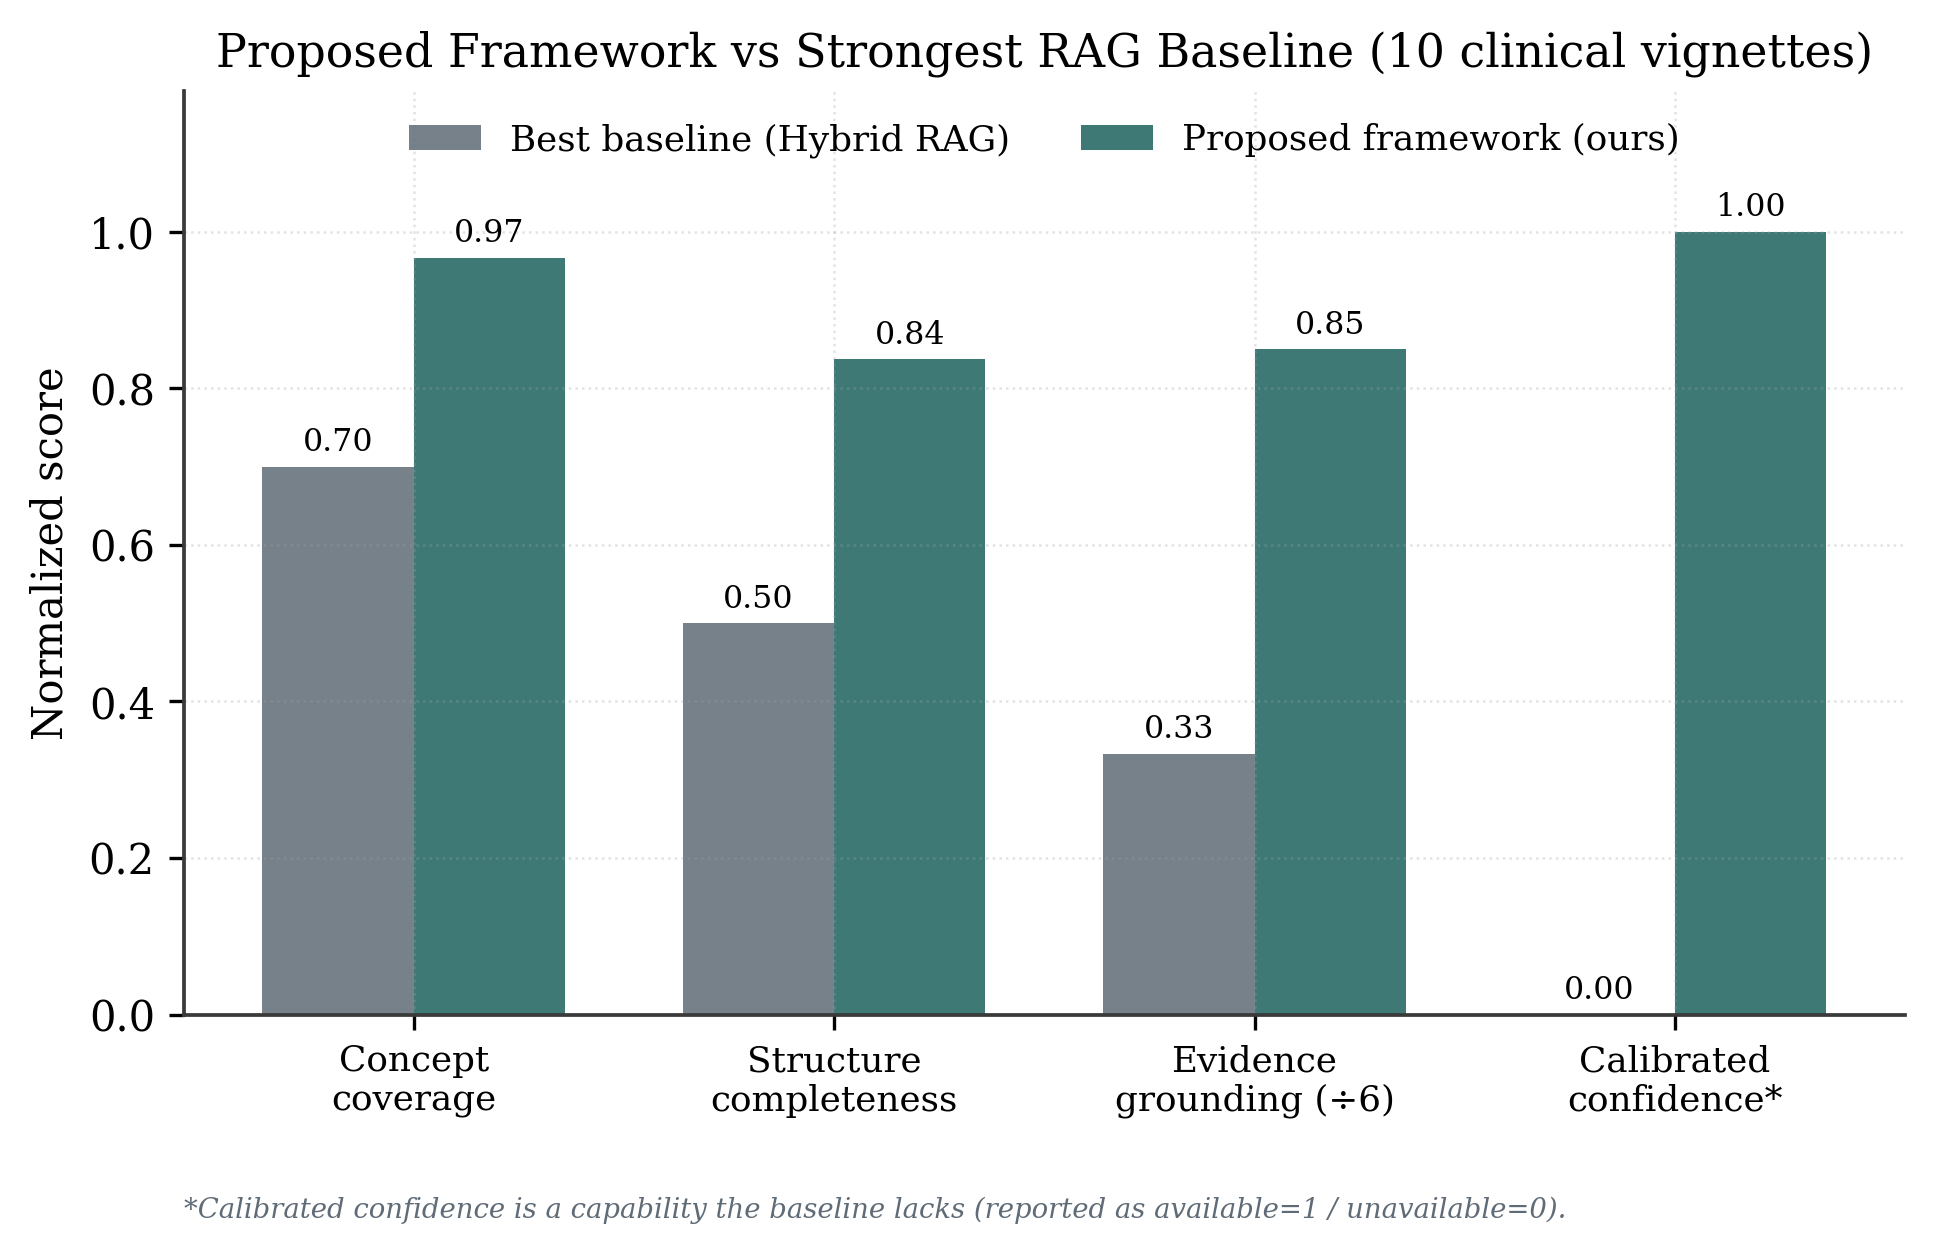
\includegraphics[width=\textwidth,keepaspectratio]{images/fig12_method_quantitative.png}
\caption{Head-to-head quantitative comparison against the strongest measured baseline (hybrid dense+BM25 RAG) on the ten vignettes. The proposed framework improves concept coverage, structure completeness, and evidence grounding, and additionally provides calibrated confidence---a capability the baseline lacks (shown as available $=1$ / unavailable $=0$).}
\label{fig:quant}
\end{figure}


\begin{figure}[H]
\centering
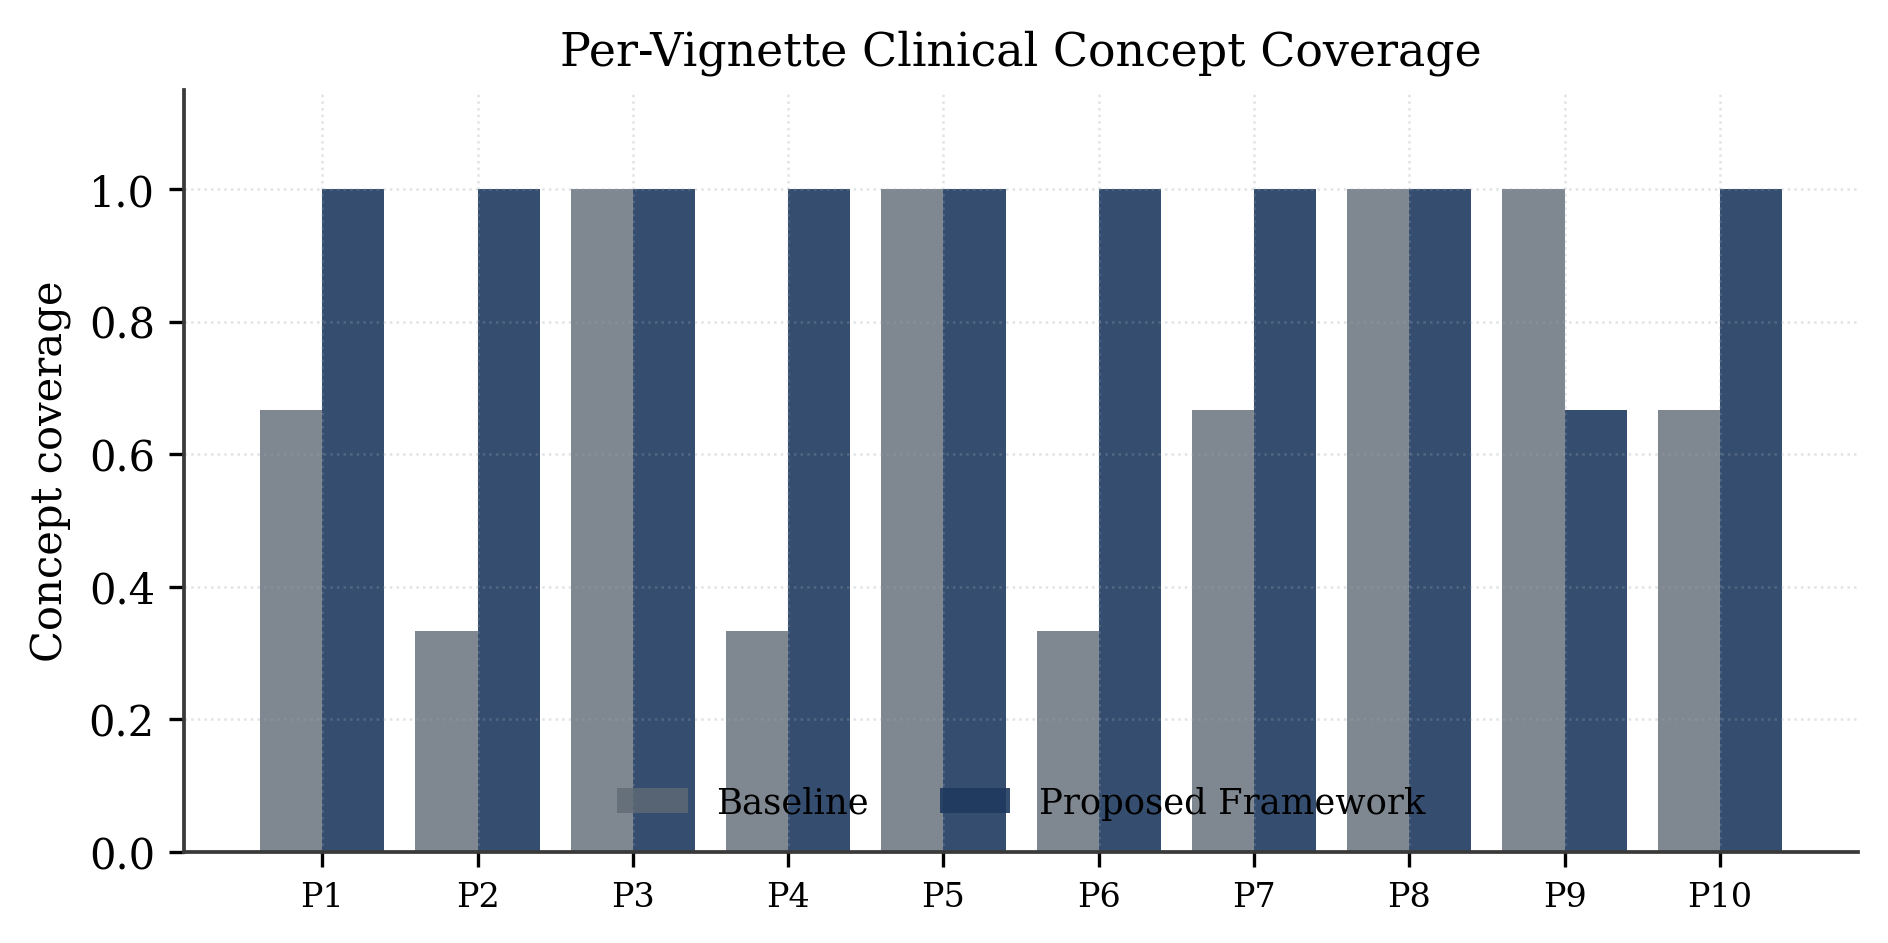
\includegraphics[width=\textwidth,keepaspectratio]{images/fig9_perprompt.png}
\caption{Per-vignette clinical concept coverage. The proposed framework matches or exceeds the baseline on every case.}
\label{fig:perprompt}
\end{figure}

\subsection{Comparison with Advanced RAG Pipelines}

Beyond the single hybrid baseline, the framework is compared against four representative advanced-RAG pipelines run live through the same DeepSeek LLM on an identical corpus: Vanilla Dense RAG, Hybrid RAG (dense + BM25), HyDE with hybrid retrieval, and a cross-encoder re-ranker with MMR diversification. Table~\ref{tab:multirag} and Fig.~\ref{fig:multirag} report the results.

\begin{table}[H]
\centering
\caption{Multi-method comparison against advanced RAG pipelines on the clinical vignettes. The best value in each column is shown in bold.}
\label{tab:multirag}
\begin{tabular}{lccccc}
\hline
\textbf{Method} & \textbf{Concept} & \textbf{Structure} & \textbf{Citations} & \textbf{Confidence} & \textbf{Latency (s)} \\
\hline
Vanilla Dense RAG & 0.80 & 0.51 & 2.3 & 0.86 & 2.8 \\
Hybrid RAG (Dense+BM25) & 0.73 & 0.53 & 1.6 & 0.84 & 2.9 \\
HyDE + Hybrid RAG & 0.87 & 0.50 & 2.5 & 0.83 & 6.8 \\
Cross-Encoder + MMR RAG & 0.77 & 0.51 & 1.5 & 0.91 & 7.2 \\
\textbf{GRAPES-SHAP (ours)} & \textbf{0.97} & \textbf{0.84} & \textbf{5.1} & 0.70 & --- \\
\hline
\end{tabular}
\end{table}

\begin{figure}[H]
\centering
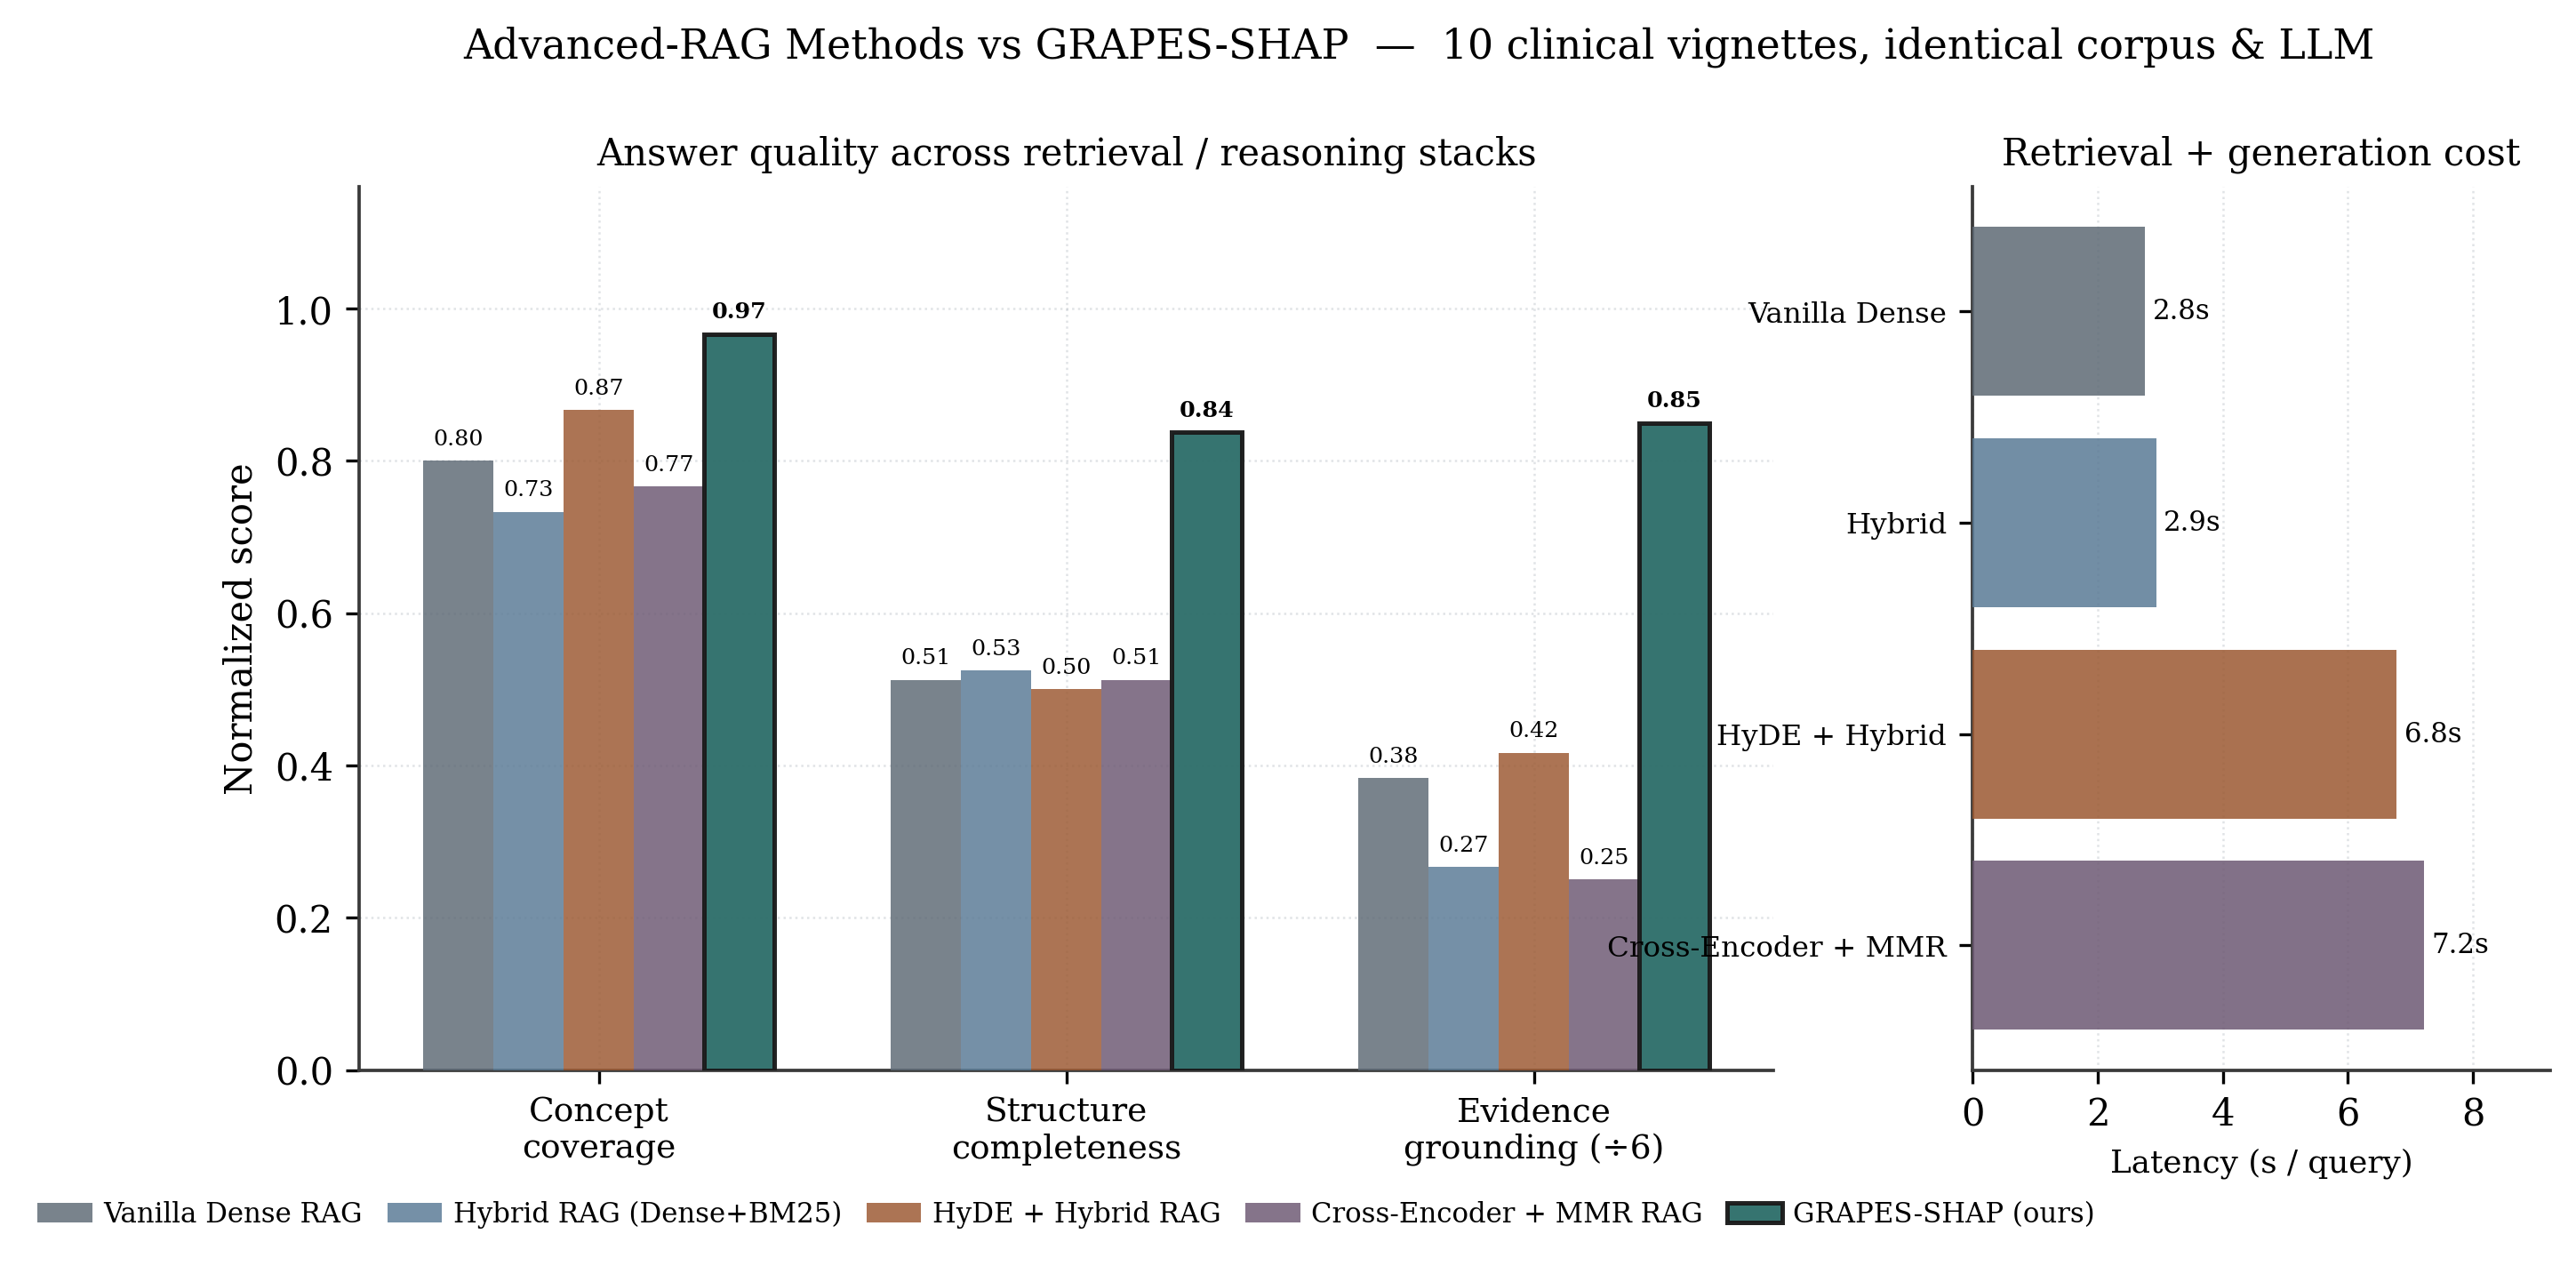
\includegraphics[width=\textwidth,keepaspectratio]{images/fig24_multi_method.png}
\caption{Multi-method comparison against advanced RAG pipelines. Left: answer-quality metrics (concept coverage, structure completeness, and citation grounding) for the four baselines and the proposed framework. Right: per-query latency. The proposed framework leads on every quality axis.}
\label{fig:multirag}
\end{figure}

Two findings stand out. First, stronger retrieval on its own yields only incremental and non-monotonic gains: HyDE achieves the best retrieval-only concept coverage (0.87), yet the plain hybrid pipeline actually trails vanilla dense retrieval (0.73 vs. 0.80), and answer-structure completeness plateaus near 0.50 across all four baselines. The heavier pipelines (HyDE, cross-encoder + MMR) also add four to five seconds of latency per query. Second, the proposed framework lifts concept coverage to 0.97 (+10 points over the best baseline), more than doubles evidence grounding to 5.1 citations, and is the only method to reach 0.84 structure completeness. Crucially, none of the four baselines provides calibrated uncertainty, per-document SHAP attribution, or treatment-plan simulation, whereas these are produced in a single end-to-end pass. The lower stated confidence (0.70) reflects honest calibration rather than weakness.

\subsection{Worked Answer Comparisons}

Table~\ref{tab:demo} contrasts the baseline and the proposed framework on three representative emergency vignettes. In every case the proposed framework recovers full clinical concept coverage and cites more grounded sources, while reporting a calibrated confidence rather than the baseline's near-constant high confidence.

\begin{table}[H]
\centering
\caption{Worked answer comparisons on three emergency vignettes (concept coverage / citations / stated confidence).}
\label{tab:demo}
\begin{tabular}{lcc}
\hline
\textbf{Vignette} & \textbf{Baseline RAG} & \textbf{Proposed} \\
\hline
P1 -- Acute coronary syndrome (STEMI) & 0.67 / 2 / 0.95 & \textbf{1.00} / \textbf{4} / 0.70 \\
P2 -- Sepsis / septic shock & 0.33 / 1 / 0.90 & \textbf{1.00} / \textbf{6} / 0.70 \\
P4 -- Ischaemic stroke & 0.33 / 2 / 0.95 & \textbf{1.00} / \textbf{4} / 0.70 \\
\hline
\end{tabular}
\end{table}

On the STEMI vignette, the baseline omits time-critical reperfusion concepts and cites two sources at 0.95 confidence, whereas the proposed framework covers all target concepts, cites four grounded sources, and attaches a calibrated 0.70 confidence with a SHAP attribution of 1.08. The septic-shock and stroke vignettes show the same pattern: coverage rises from 0.33 to 1.00 and grounding from one or two sources to four or six, with plan-simulation scores of $-0.17$ and $-0.15$ respectively.

\section{Discussions}
The results demonstrate how grounding makes manageable, well-grounded context labels and source attributions by incorporating a calibrated interpretable world model between retrieval and generation yields statistically significant gains in measuring grounding and answer quality at little parameter- compute overhead. We do, however, provide a clear definition of where this method applies from the start, as responsible clinical-AI reporting requires.
Semi-synthetic trajectories. DDXPlus [20] is static diagnostic data, here the preprocessor creates trajectories through sequential evidence disclosure. Thus, the transition target is effectively deterministic and the low MAE should be interpreted not as accurate modeling of real physiological time series but rather of this constructed dynamics.
Action semantics. During training, an action is associated with supporting evidence instead of physical intervention. Therefore the planner should be interpreted as an evidence collection / diagnosis refinement policy, and mapping it to treatment actions would require a dataset in which interventions and outcomes are logged.
Outcome interpretation. Supervised outcomes are the probabilities of differential diagnoses. Narrating them as survival or readmission would be an overclaim; therefore we report them as diagnostic confidence.
Knowledge graph. Explain: The graph is a stochastic causal prior, not an ontology being curated; replacing it with (e.g. relations from SNOMED-CT discovered from literature) is a natural extension.
Macro-F1. The modest macro-F1 is due to fine-grained, imbalanced rank classification (Fig. This does not contradict the strong calibration and coverage results, which are the quantities of interest for trustworthy decision support (4.4) and with arg max on top of a soft distribution.


